\documentclass[../../main.tex]{subfiles}
\begin{document}
\section{Validity of a Two-dimensional beam} \label{sec:validity-of-a-cantilever-timoshenko-beam}
This section is an extention of section \ref{sec:validity-of-a-cantilever-timoshenko-beam} and the article \cite{LVV09}. As seen in the previous section, the two-dimensional model does have some characteristics that are not related to beam-type problems. This is also true for the three-dimensional model. 

The results in this section will show that the three-dimensional model has a lot of non-beam type eigenvalues. It is due to this reason, the authors of \cite{LVV09} suggested to use the two-dimensional model as an intermediate step. The the previous section, the validity of a cantilever Timoshenko beam was investigated using a cantilever two-dimensional beam as a reference. In this section, the validity of a cantilever two-dimensional beam will be investigated using a cantilever three-dimensional beam as a reference.

\subsection{The models}
The two-dimensional model is the same model as used in the previous section, Problem T-2 defined in section \ref{ssec:2D_Model:ModelProblem}. From section \ref{ssec:3D_Model:ModelProblems}, the cantilever three-dimensional model, referred to as Problem 3D-1.

Figure \ref{fig:2Dv3D} shows the two beams side-by-side.

\FloatBarrier
\begin{figure}[h!]
	\scalebox{.8}{
		\makebox[\textwidth][c]{
			\caption{Side-by-side comparison of the beams.}
			\label{fig:2Dv3D}
			\centering
			\begin{minipage}[b]{0.7\linewidth}
				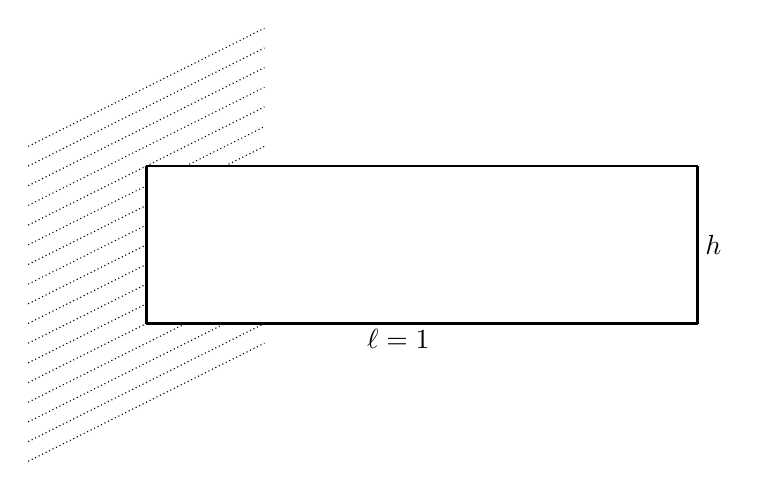
\begin{tikzpicture}
					\draw[line width = 0.3mm] (0,1) -- (7,1);
					\draw[line width = 0.3mm] (0,-1) -- (7,-1);
					\draw[line width = 0.3mm] (7,-1) -- (7,1);
					\draw[line width = 0.3mm] (0,-1) -- (0,1);
					
					
					\draw[scale=0.5, domain=-3:3, smooth, variable=\x,densely dotted] plot ({\x}, {0.5*\x+4});
					\draw[scale=0.5, domain=-3:3, smooth, variable=\x,densely dotted] plot ({\x}, {0.5*\x+3.5});
					\draw[scale=0.5, domain=-3:3, smooth, variable=\x,densely dotted] plot ({\x}, {0.5*\x+3});
					\draw[scale=0.5, domain=-3:3, smooth, variable=\x,densely dotted] plot ({\x}, {0.5*\x+2.5});
					\draw[scale=0.5, domain=-3:3, smooth, variable=\x,densely dotted] plot ({\x}, {0.5*\x+2});
					
					\draw[scale=0.5, domain=-3:0, smooth, variable=\x,densely dotted] plot ({\x}, {0.5*\x+1.5});
					\draw[scale=0.5, domain=-3:0, smooth, variable=\x,densely dotted] plot ({\x}, {0.5*\x+1});
					
					
					\draw[scale=0.5, domain=1:3, smooth, variable=\x,densely dotted] plot ({\x}, {0.5*\x+1.5});
					\draw[scale=0.5, domain=2:3, smooth, variable=\x,densely dotted] plot ({\x}, {0.5*\x+1});
					
					\draw[scale=0.5, domain=-3:0, smooth, variable=\x,densely dotted] plot ({\x}, {0.5*\x+0.5});
					\draw[scale=0.5, domain=-3:0, smooth, variable=\x,densely dotted] plot ({\x}, {0.5*\x});
					\draw[scale=0.5, domain=-3:0, smooth, variable=\x,densely dotted] plot ({\x}, {0.5*\x-0.5});
					\draw[scale=0.5, domain=-3:0, smooth, variable=\x,densely dotted] plot ({\x}, {0.5*\x-1});
					\draw[scale=0.5, domain=-3:0, smooth, variable=\x,densely dotted] plot ({\x}, {0.5*\x-1.5});
					\draw[scale=0.5, domain=-3:0, smooth, variable=\x,densely dotted] plot ({\x}, {0.5*\x-2});
					\draw[scale=0.5, domain=-3:1, smooth, variable=\x,densely dotted] plot ({\x}, {0.5*\x-2.5});
					\draw[scale=0.5, domain=-3:2, smooth, variable=\x,densely dotted] plot ({\x}, {0.5*\x-3});
					\draw[scale=0.5, domain=-3:3, smooth, variable=\x,densely dotted] plot ({\x}, {0.5*\x-3.5});
					\draw[scale=0.5, domain=-3:3, smooth, variable=\x,densely dotted] plot ({\x}, {0.5*\x-4});
					
					\node at (7.2,0) {$h$};
					\node at (3.2,-1.2) {$\ell = 1$};
				\end{tikzpicture}
				\subcaption{Two-Dimensional Elastic Body}
			\end{minipage}
			\begin{minipage}[b]{0.7\linewidth}
				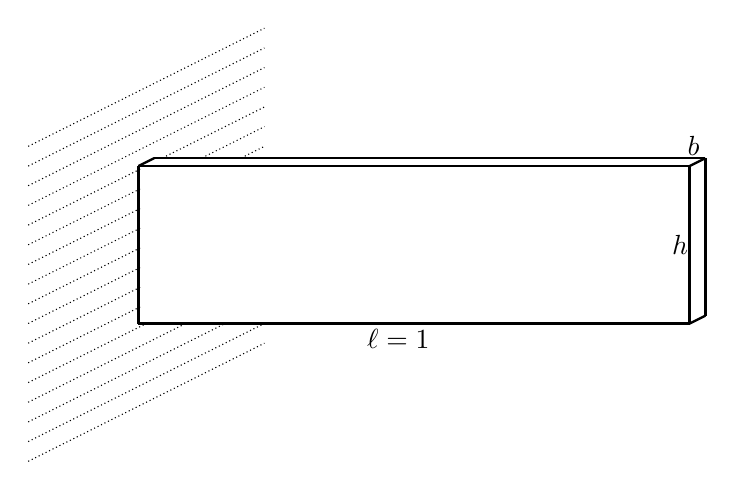
\begin{tikzpicture}
					\draw[line width = 0.3mm] (-0.1,1) -- (6.9,1);
					\draw[line width = 0.3mm] (-0.1,-1) -- (6.9,-1);
					\draw[line width = 0.3mm] (6.9,-1) -- (6.9,1);
					\draw[line width = 0.3mm] (-0.1,-1) -- (-0.1,1);
					
					\draw[line width = 0.3mm] (0.1,1.1) -- (7.1,1.1);
					\draw[line width = 0.3mm] (7.1,-0.9) -- (7.1,1.1);
					
					\draw[line width = 0.3mm] (-0.1,1) -- (0.1,1.1);
					\draw[line width = 0.3mm] (6.9,1) -- (7.1,1.1);
					\draw[line width = 0.3mm] (6.9,-1) -- (7.1,-0.9);
					
					
					
					\draw[scale=0.5, domain=-3:3, smooth, variable=\x,densely dotted] plot ({\x}, {0.5*\x+4});
					\draw[scale=0.5, domain=-3:3, smooth, variable=\x,densely dotted] plot ({\x}, {0.5*\x+3.5});
					\draw[scale=0.5, domain=-3:3, smooth, variable=\x,densely dotted] plot ({\x}, {0.5*\x+3});
					\draw[scale=0.5, domain=-3:3, smooth, variable=\x,densely dotted] plot ({\x}, {0.5*\x+2.5});
					
					\draw[scale=0.5, domain=-3:-0.1, smooth, variable=\x,densely dotted] plot ({\x}, {0.5*\x+2});
					\draw[scale=0.5, domain=-3:-0.1, smooth, variable=\x,densely dotted] plot ({\x}, {0.5*\x+1.5});
					\draw[scale=0.5, domain=-3:-0.1, smooth, variable=\x,densely dotted] plot ({\x}, {0.5*\x+1});
					
					\draw[scale=0.5, domain=0.5:3, smooth, variable=\x,densely dotted] plot ({\x}, {0.5*\x+2});
					\draw[scale=0.5, domain=1.5:3, smooth, variable=\x,densely dotted] plot ({\x}, {0.5*\x+1.5});
					\draw[scale=0.5, domain=2.5:3, smooth, variable=\x,densely dotted] plot ({\x}, {0.5*\x+1});
					
					\draw[scale=0.5, domain=-3:-0.1, smooth, variable=\x,densely dotted] plot ({\x}, {0.5*\x+0.5});
					\draw[scale=0.5, domain=-3:-0.1, smooth, variable=\x,densely dotted] plot ({\x}, {0.5*\x});
					\draw[scale=0.5, domain=-3:-0.1, smooth, variable=\x,densely dotted] plot ({\x}, {0.5*\x-0.5});
					\draw[scale=0.5, domain=-3:-0.1, smooth, variable=\x,densely dotted] plot ({\x}, {0.5*\x-1});
					\draw[scale=0.5, domain=-3:-0.1, smooth, variable=\x,densely dotted] plot ({\x}, {0.5*\x-1.5});
					\draw[scale=0.5, domain=-3:0, smooth, variable=\x,densely dotted] plot ({\x}, {0.5*\x-2});
					\draw[scale=0.5, domain=-3:1, smooth, variable=\x,densely dotted] plot ({\x}, {0.5*\x-2.5});
					\draw[scale=0.5, domain=-3:2, smooth, variable=\x,densely dotted] plot ({\x}, {0.5*\x-3});
					\draw[scale=0.5, domain=-3:3, smooth, variable=\x,densely dotted] plot ({\x}, {0.5*\x-3.5});
					\draw[scale=0.5, domain=-3:3, smooth, variable=\x,densely dotted] plot ({\x}, {0.5*\x-4});
					
					\node at (6.95,1.25) {$b$};
					\node at (6.78,0) {$h$};
					\node at (3.2,-1.2) {$\ell = 1$};
					

				\end{tikzpicture}
				\subcaption{Three-Dimensional Elastic Body}
				
			\end{minipage}
		}
	}
\end{figure}
\FloatBarrier

\subsection{Calculating the eigenvalues}
Similar to calculating the eiegnvalues of the two-dimensional beam, to calculate the eigenvalues of the three-dimensional beam, the Finite Element Method is used. In section \ref{sec:FEM:3D}, the Finite Element Method for the three-dimensional beam is derived. Section \ref{3dFEM_EP} gives the following eigenvalue problem for the three-dimensional beam:

\subsubsection{Problem 3D-1E}
Find a real number $\lambda$ and a function $\bar{u} \in S^h$ such that
\begin{eqnarray}
	K\bar{u} & = & M\lambda{\bar{u}},
\end{eqnarray} where $K$ and $M$ are the standard Finite Element Matrices for tri-cubic basis functions. The definition of the matrices are given in section \ref{sec:FEM:3D}.

\subsubsection{Accuracy of the eigenvalues}
Figure \ref{fig:conv_3d_eig} show the rate of convergence of the first 20 eigenvalues of Problem 3D-1E. 

\begin{figure}[H]
    \centering
    \begin{adjustbox}{center}
        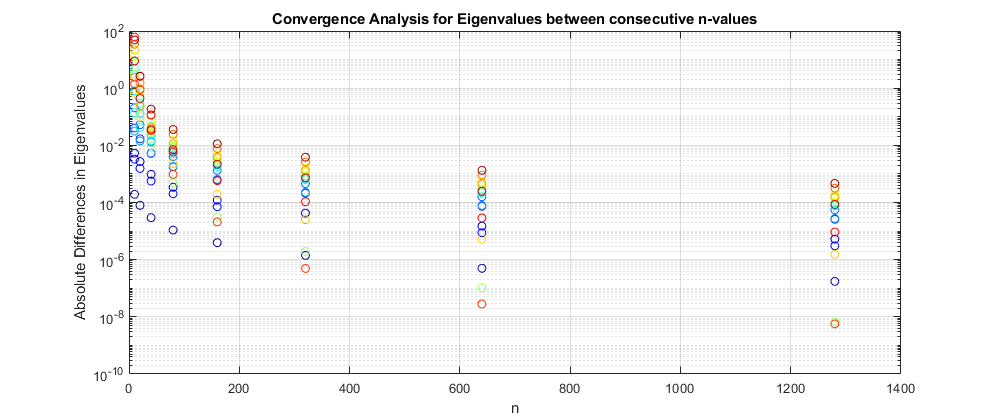
\includegraphics[scale=0.7]{Convergence.png}
    \end{adjustbox}
    \caption{Rate of convergence of the first 20 eigenvalues.}
    \label{fig:conv_3d_eig}
\end{figure}
\textcolor{red}{Update this figure.}

Similar to the two-dimensional case, the number of elements can be chosen so that at least the first 10 eigenvalues are accurate to 5 significant digits.

\subsection{Comparing the mode shapes}
The method to match up the eigenvalues remains the same as in the previous section. Since the three-dimensional model is more complex, there are more mode shapes that do no appear in the Timoshenko model or two-dimensional model. The focus remains on beam-type problems, so the mode shapes relating to beam type problems are most important.

\subsubsection{Mode shapes relating to beam type eigenvalues.}
Figure \ref{fig:beam-2dv3d} show some examples of beam type mode shapes for the displacement $u$.

\begin{figure}[h!]
	\scalebox{.8}{
		\makebox[\textwidth][c]{
			\centering
			\begin{minipage}[b]{0.8\linewidth}
				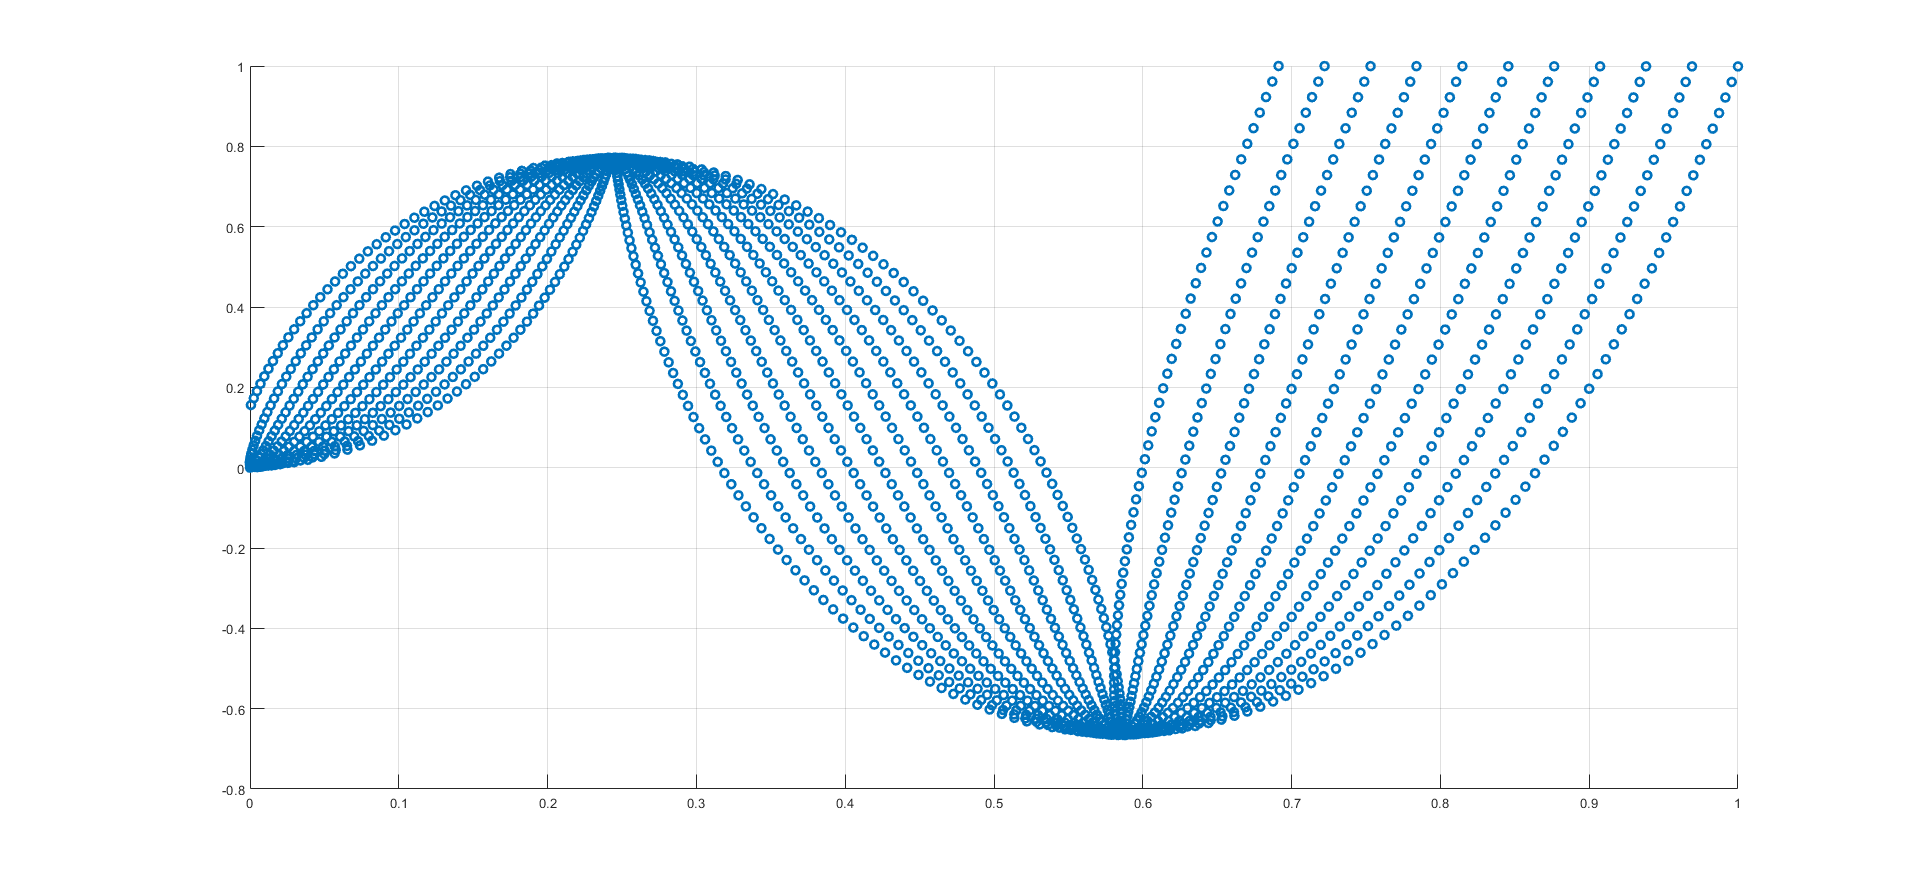
\includegraphics[width=1\linewidth]{3D12.png}
				\subcaption{3D Beam Type - $\lambda_{12} = 2.3293$}
				\label{fig:minipage2}
			\end{minipage}
			\begin{minipage}[b]{0.8\linewidth}
				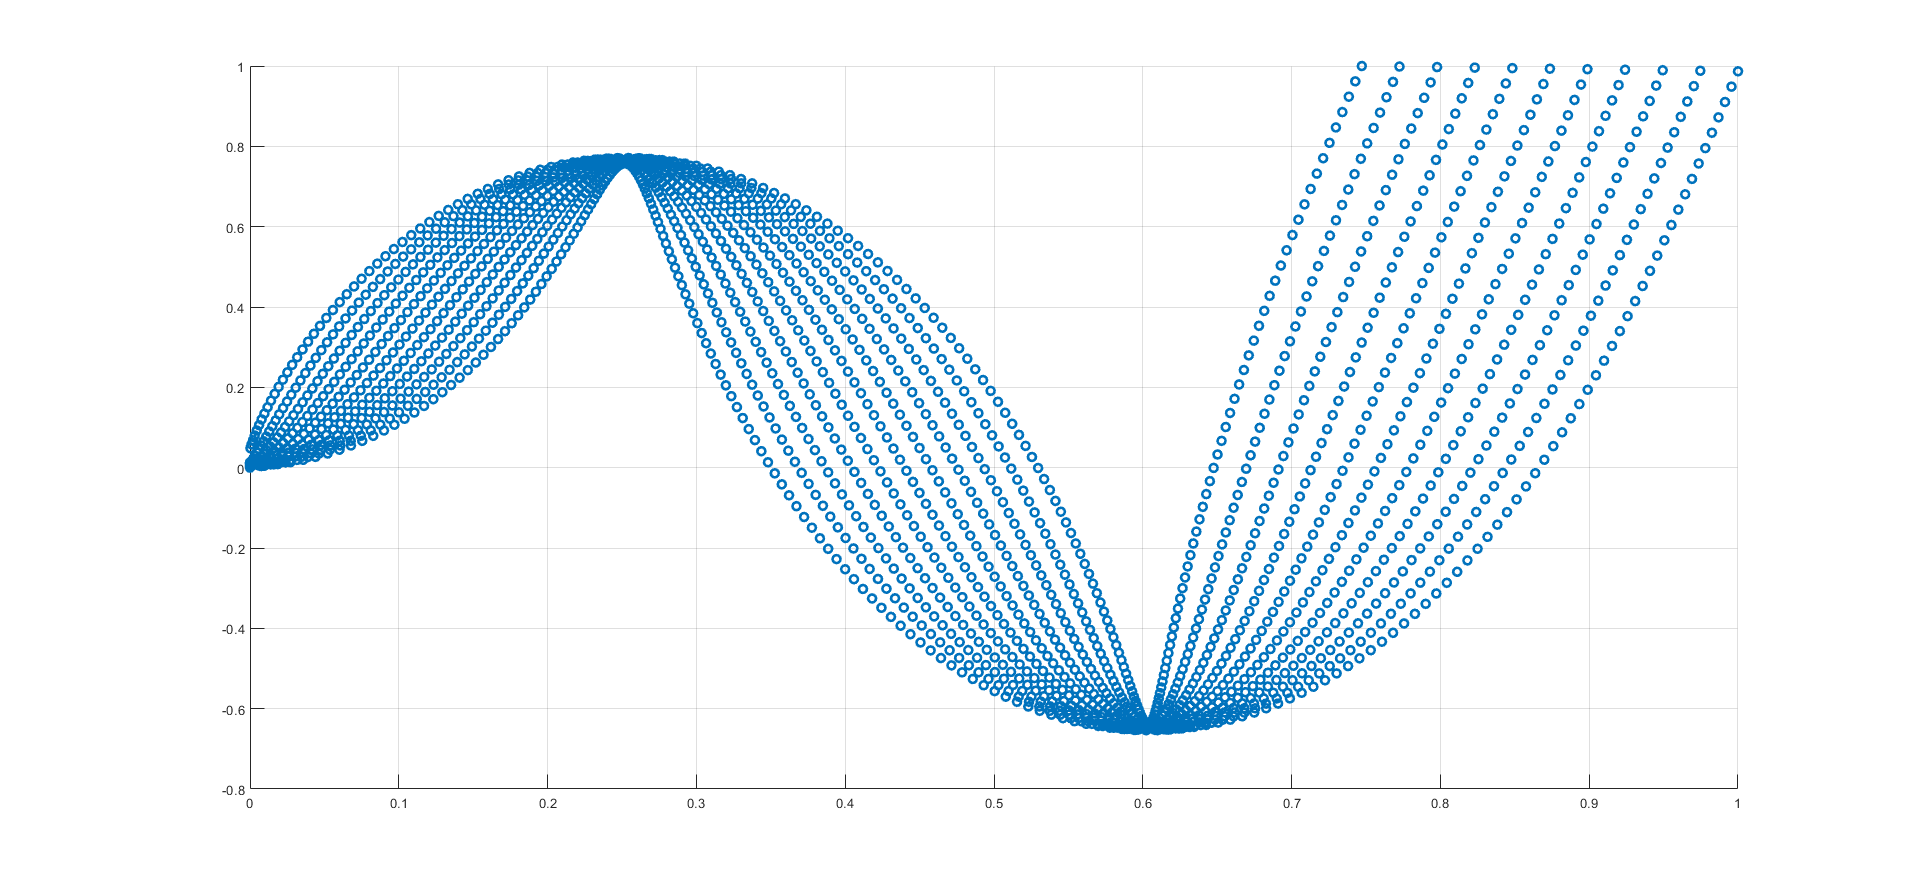
\includegraphics[width=1\linewidth]{2D3.png}
				\subcaption{2D Beam Type - $\lambda_3 = 2.3273$}
				\label{fig:minipage1}
			\end{minipage}
	}}
	\scalebox{.8}{
		\makebox[\textwidth][c]{
			\centering
			\begin{minipage}[b]{0.8\linewidth}
				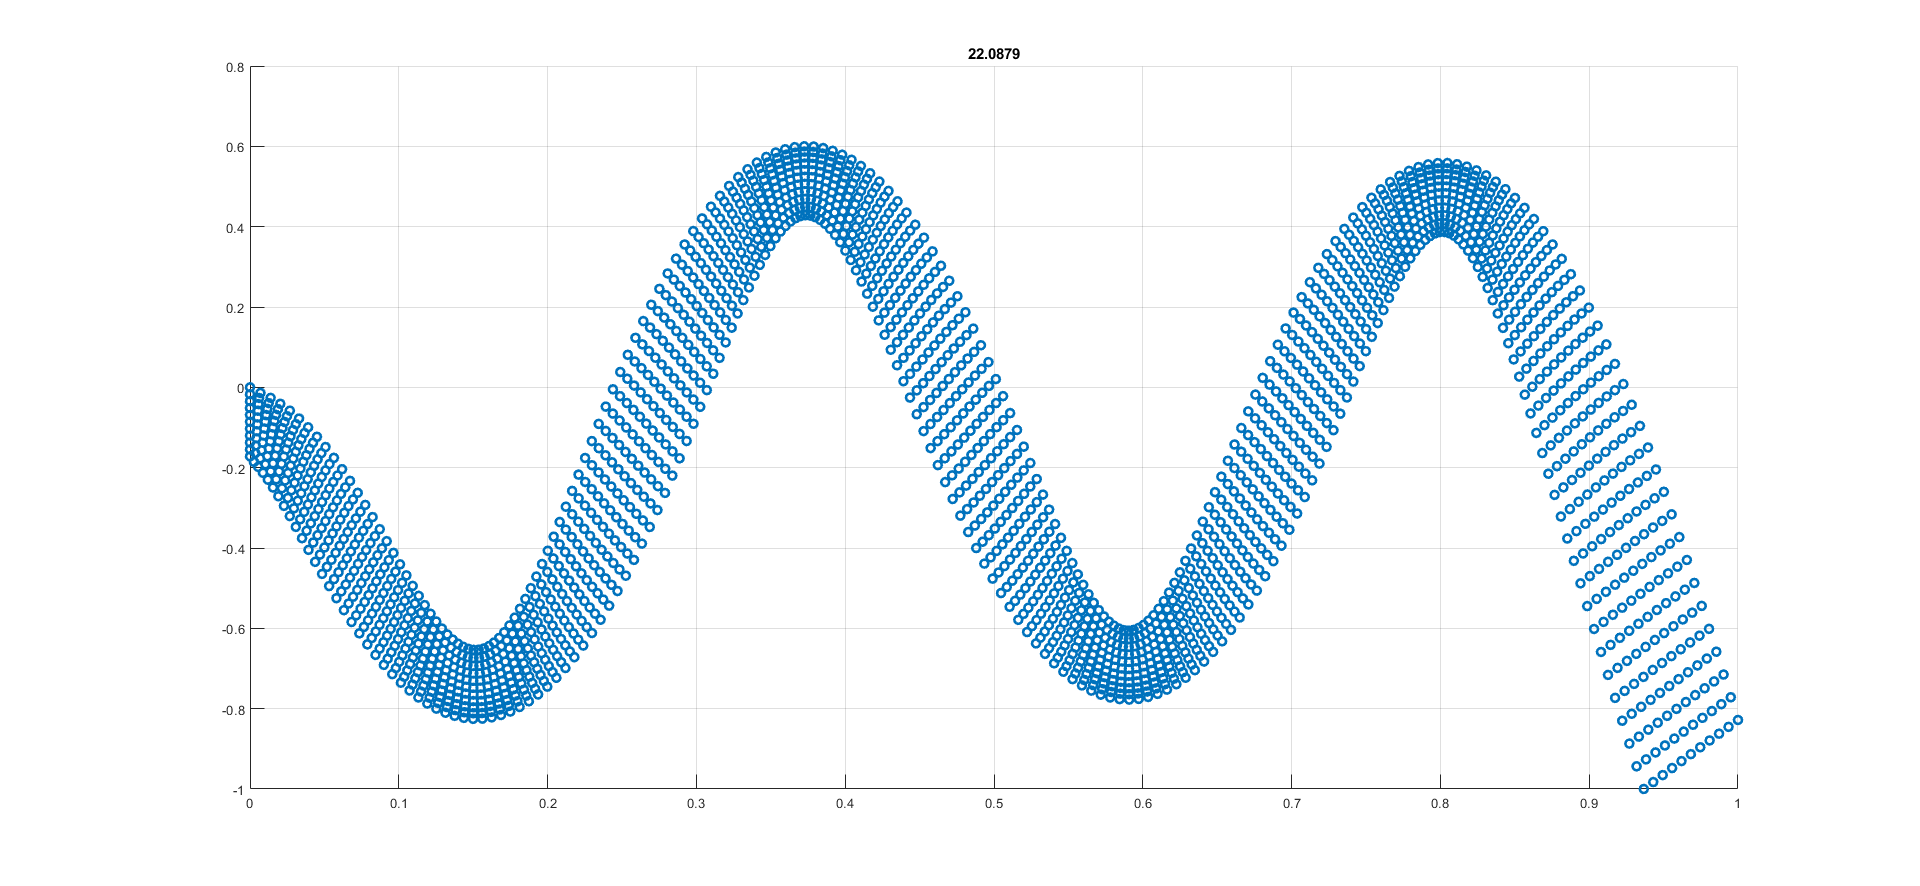
\includegraphics[width=1\linewidth]{3D22.png}
				\subcaption{3D Beam Type - $\lambda_{24} = 21.929$}
				\label{fig:minipage2}
			\end{minipage}
			\begin{minipage}[b]{0.8\linewidth}
				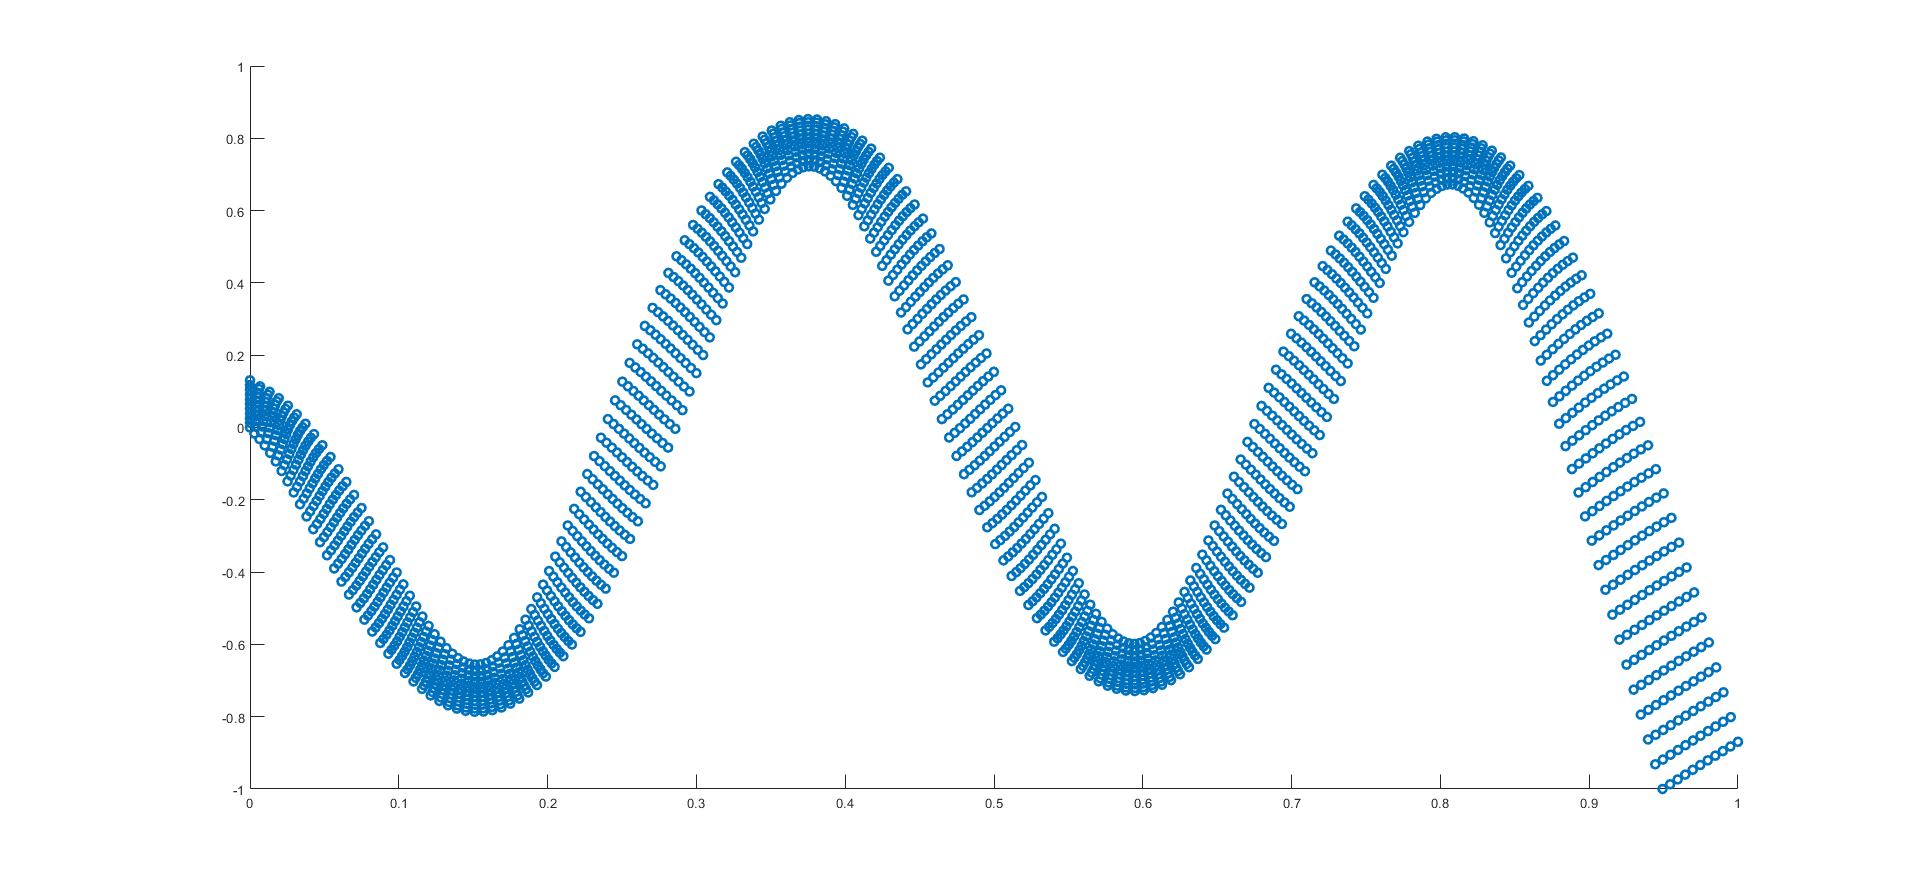
\includegraphics[width=1\linewidth]{2D6.png}
				\subcaption{2D Beam Type - $\lambda_6 = 21.911$}
				\label{fig:minipage1}
			\end{minipage}
			\caption{Mode shapes of the displacement $w$ with $h=1/20$.}
			\label{fig:beam-2dv3d}
	}}
\end{figure}
\FloatBarrier

\subsubsection{Mode shapes relating to non-beam type eigenvalues that are present in the two-dimensional model.}
Figure \ref{fig:nonbeam-2dv3d} show examples of mode shapes relating to non-beam type eigenvalues for the displacement $u$.

\FloatBarrier
\begin{figure}[h!]
	\scalebox{.8}{
		\makebox[\textwidth][c]{
			\centering
			\begin{minipage}[b]{0.8\linewidth}
				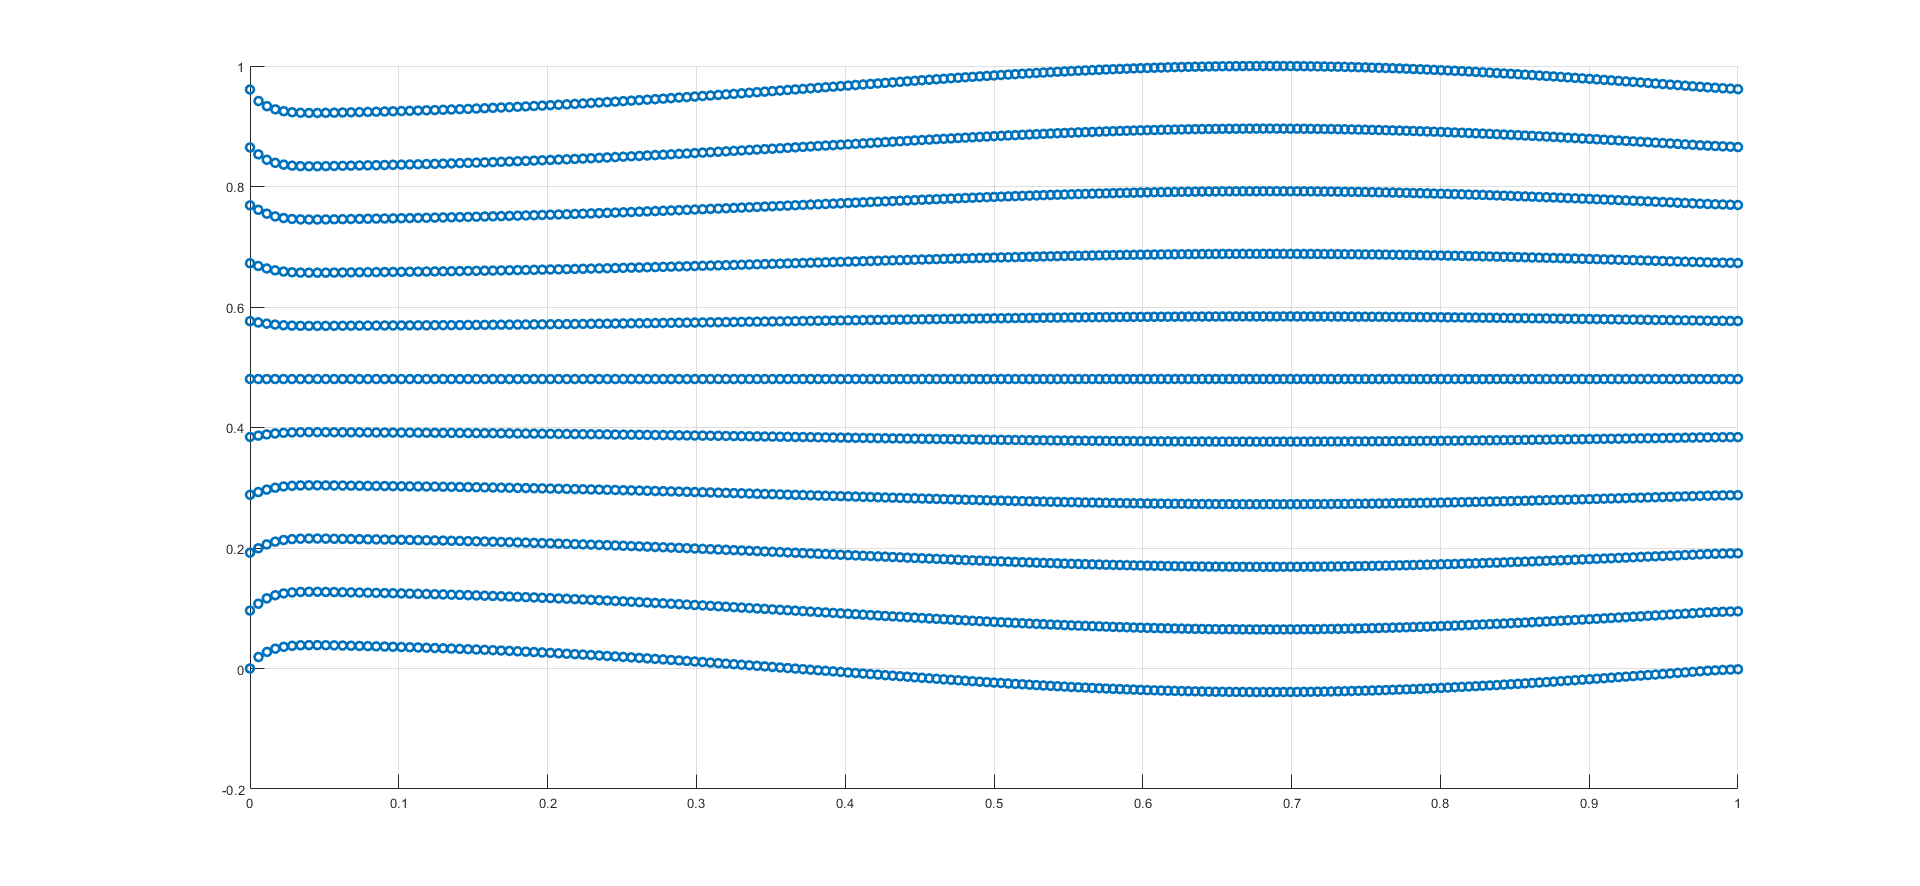
\includegraphics[width=1\linewidth]{3D33.png}
				\subcaption{3D Non-Beam Type - $\lambda_{33} = 69.374$}
				\label{fig:minipage2}
			\end{minipage}
			\begin{minipage}[b]{0.8\linewidth}
				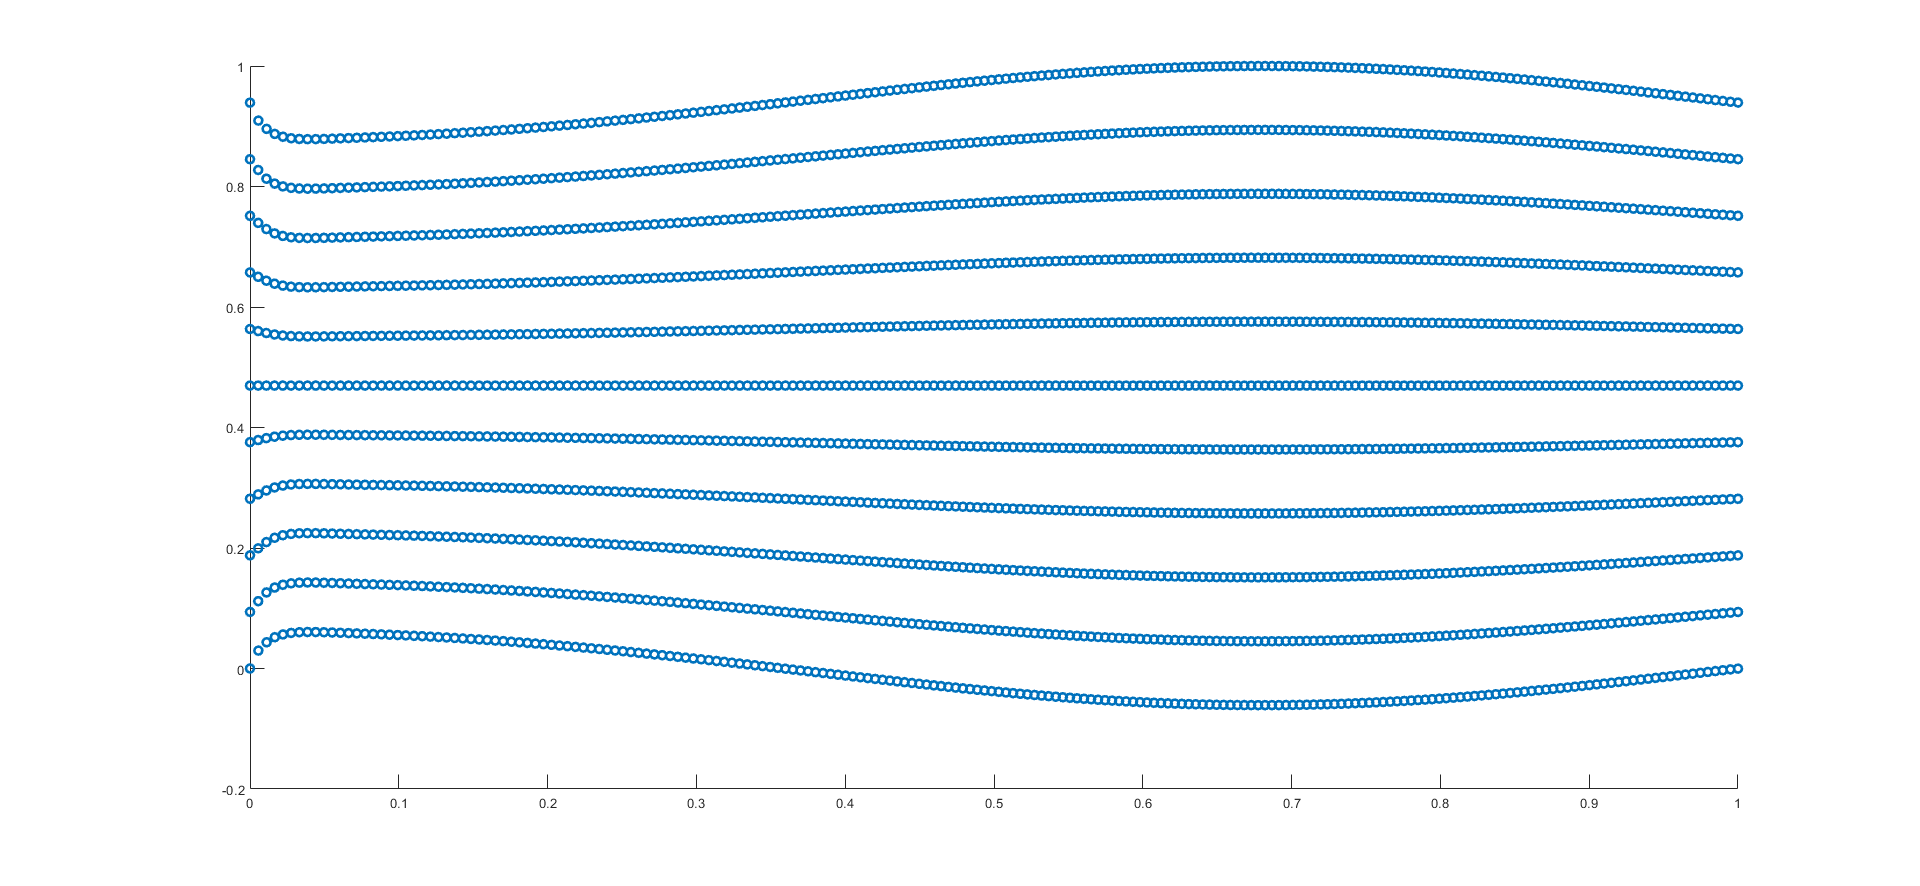
\includegraphics[width=1\linewidth]{2D8.png}
				\subcaption{2D Non-Beam Type - $\lambda_8 = 69.344$}
				\label{fig:minipage1}
			\end{minipage}
			\caption{Mode shapes of the displacement $w$ with $h=1/20$.}
			\label{fig:nonbeam-2dv3d}
	}}
\end{figure}
\FloatBarrier

\subsubsection{Mode shapes relating to non-beam type eigenvalues that are not present in the two-dimensional model.}
Figure \ref{fig:nonbeam-2dv3d} show examples of mode shapes relating to non-beam type eigenvalues for the displacement $u$ which are not present in the two-dimensional model. These mode shapes only appear in the three-dimensional beam.
\FloatBarrier
\begin{figure}[h!]
	\scalebox{.8}{
		\makebox[\textwidth][c]{
			\centering
			\begin{minipage}[b]{0.8\linewidth}
				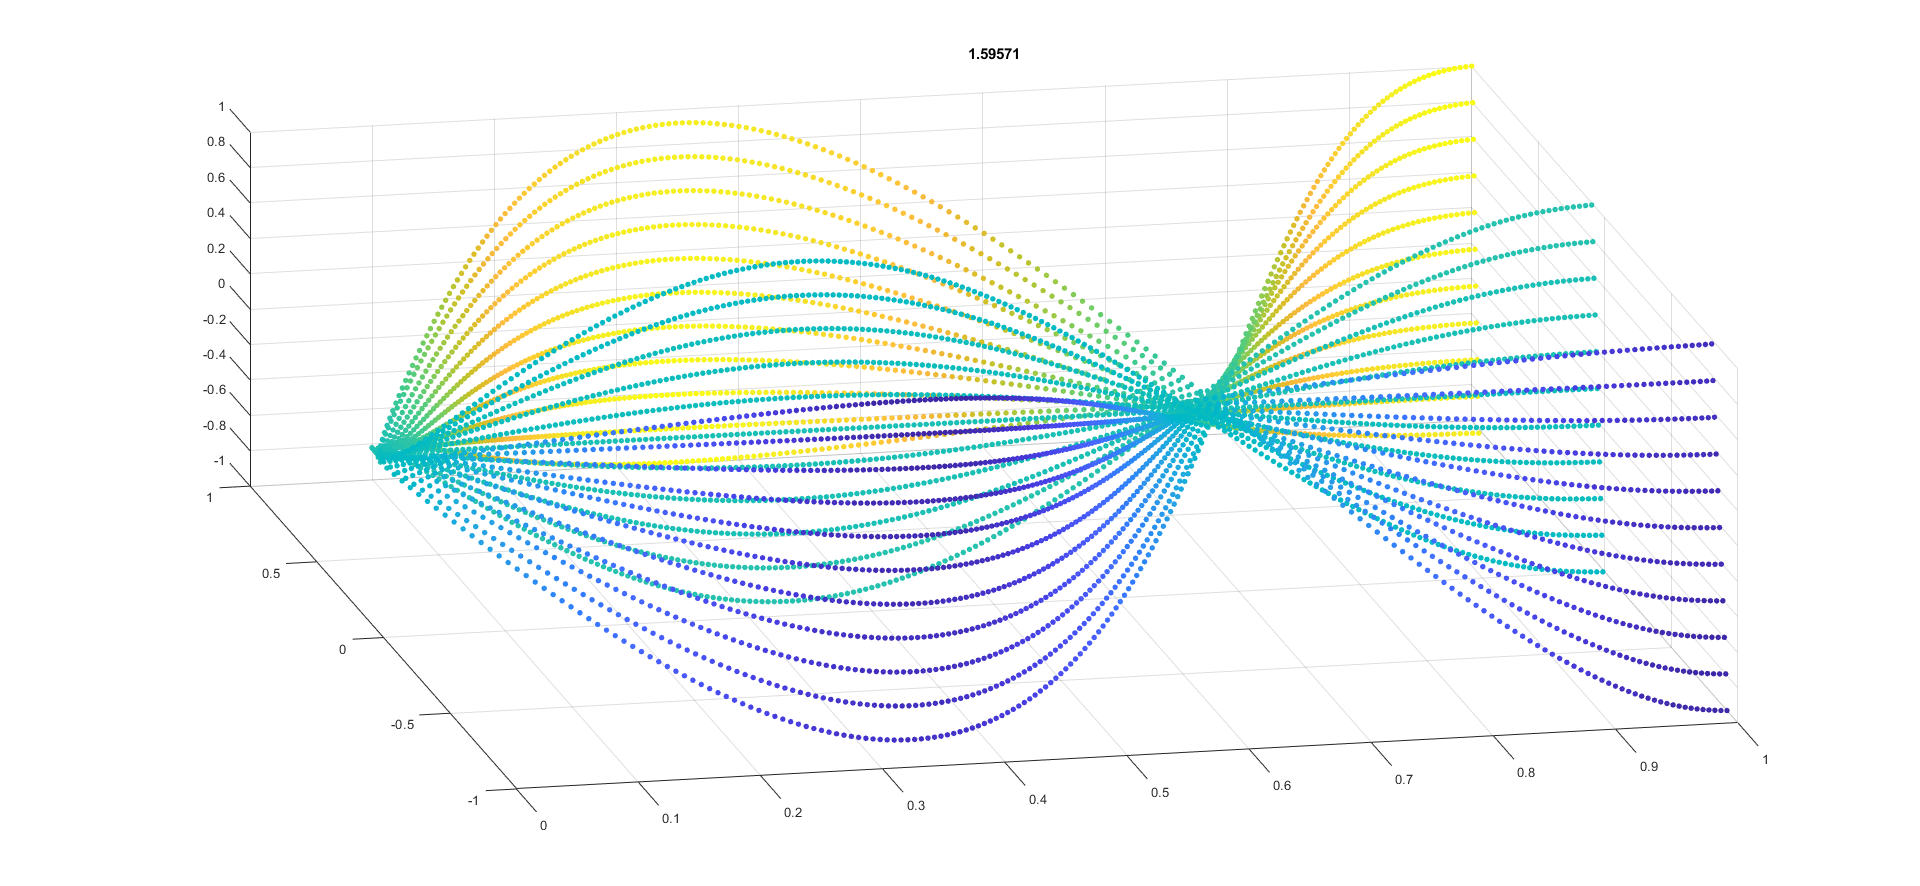
\includegraphics[width=1\linewidth]{3DNonBeam10.png}
				\subcaption{Non-2D Type - $\lambda_{10}$}
				\label{fig:minipage2}
			\end{minipage}
			\begin{minipage}[b]{0.8\linewidth}
				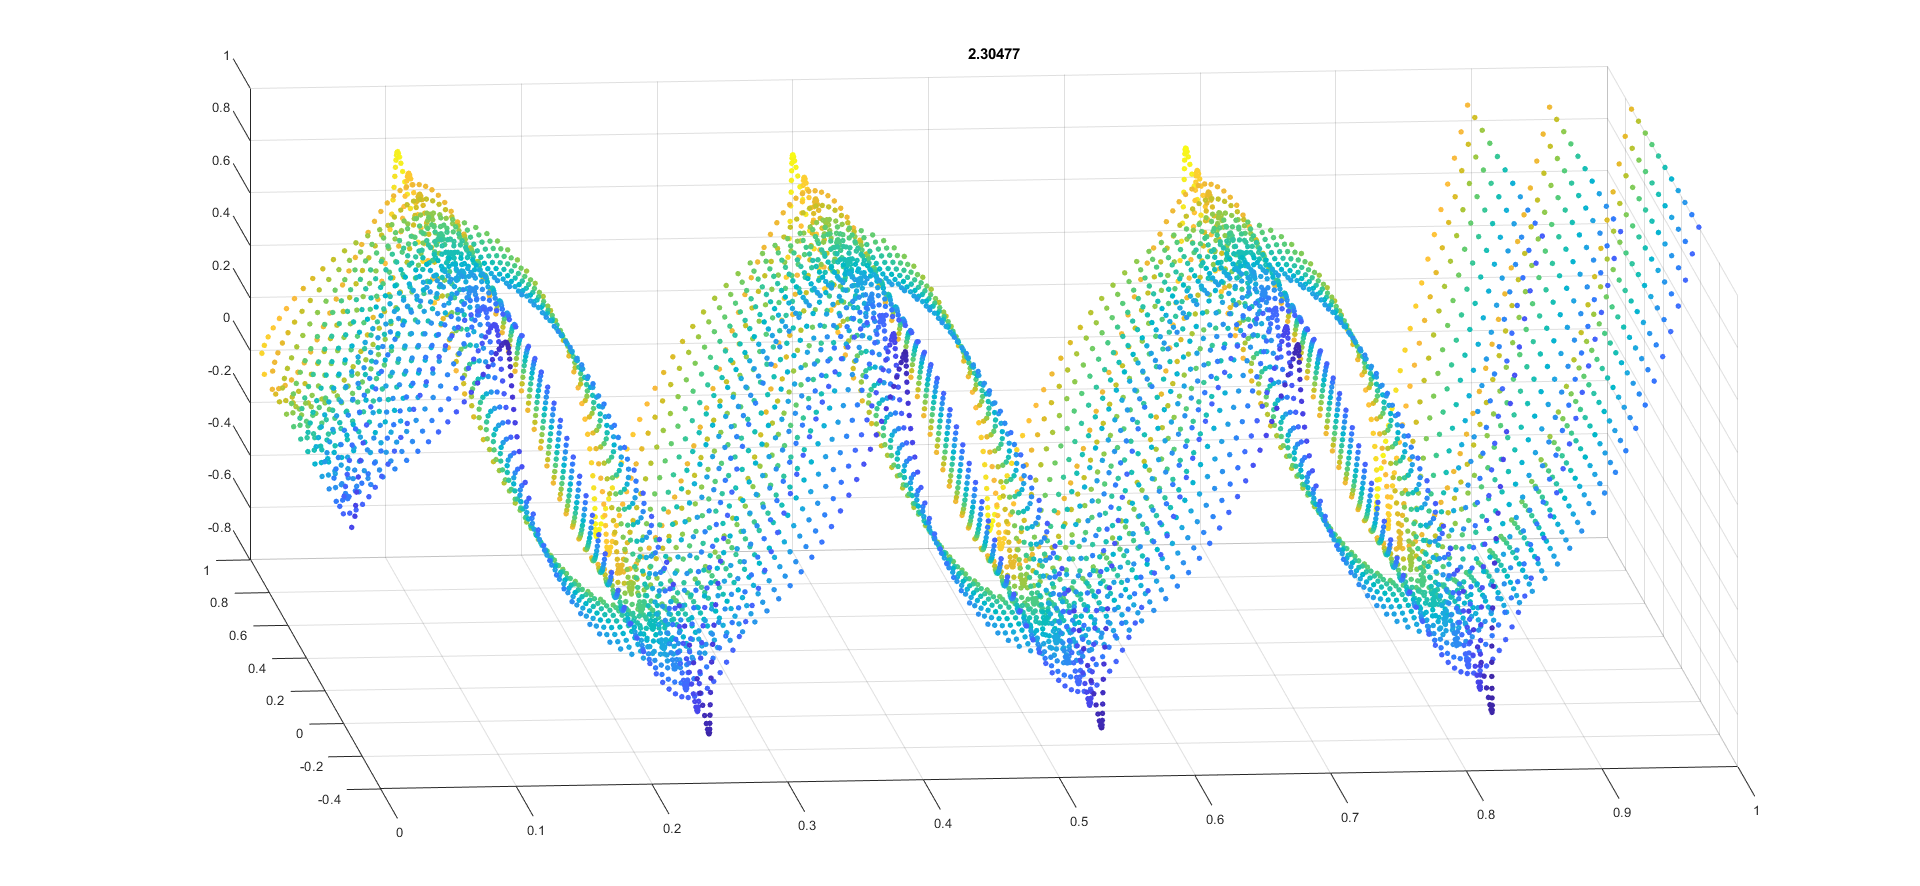
\includegraphics[width=1\linewidth]{3DNonBeam11.png}
				\subcaption{Non-2D Type - $\lambda_{11}$}
				\label{fig:minipage11}
			\end{minipage}
			\caption{Mode shapes of the displacement $w$ with $\alpha = 4800$.}
			
	}}
\end{figure}
\FloatBarrier

\subsection{Comparing the eigenvalues}
The eigenvalues of the two models can now be compared. Recall from the introduction, that the two-dimensional and three-dimensional models have different paramaters.

The two-dimensional model has the single paramater $h$ representing the height of the beam. The three-dimensional model has two parameters, $h$ and $b$, representing the height and width of the beam respectively.  


\end{document}